% Generated by AP Math GOLD PILOT deterministic Python generator.
% input id: H02_point_tangent
\documentclass{article}
\usepackage[margin=1cm]{geometry}
\def\pgfsysdriver{pgfsys-dvisvgm.def}
\usepackage{fontspec}
\setmainfont{Malgun Gothic}
\setsansfont{Malgun Gothic}
\usepackage{amsmath}
\usepackage{amssymb}
\usepackage{pgfplots}
\pgfplotsset{compat=1.18}
\pagestyle{empty}
\begin{document}
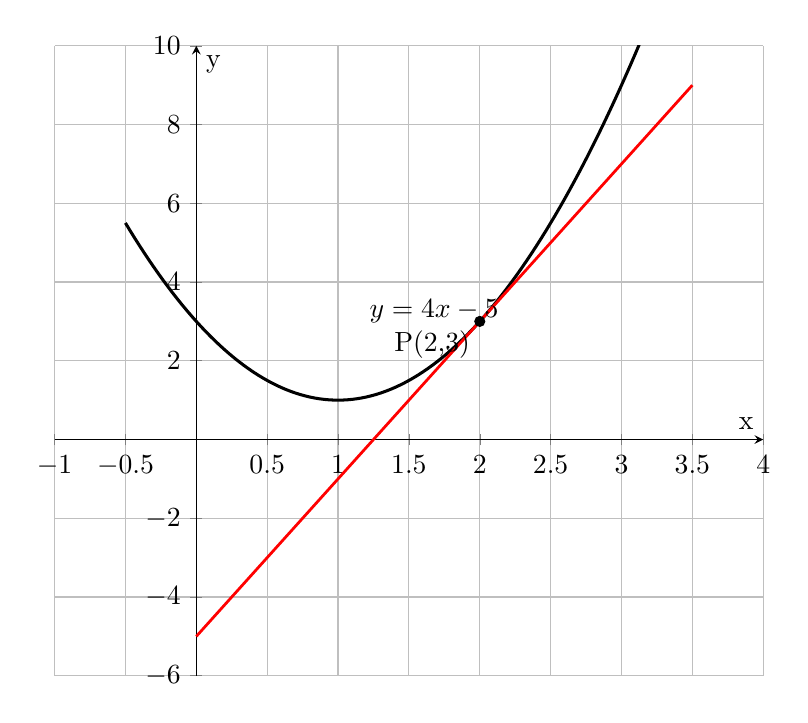
\begin{tikzpicture}
\begin{axis}[width=9cm,height=8cm,scale only axis,axis lines=middle,grid=major,xmin=-1,xmax=4,ymin=-6,ymax=10,xlabel={x},ylabel={y},clip=true]
\addplot[black, solid, line width=1.1pt] coordinates {(-0.5,5.5) (-0.466667,5.302222) (-0.433333,5.108889) (-0.4,4.92) (-0.366667,4.735556) (-0.333333,4.555556) (-0.3,4.38) (-0.266667,4.208889) (-0.233333,4.042222) (-0.2,3.88) (-0.166667,3.722222) (-0.133333,3.568889) (-0.1,3.42) (-0.066667,3.275556) (-0.033333,3.135556) (0,3) (0.033333,2.868889) (0.066667,2.742222) (0.1,2.62) (0.133333,2.502222) (0.166667,2.388889) (0.2,2.28) (0.233333,2.175556) (0.266667,2.075556) (0.3,1.98) (0.333333,1.888889) (0.366667,1.802222) (0.4,1.72) (0.433333,1.642222) (0.466667,1.568889) (0.5,1.5) (0.533333,1.435556) (0.566667,1.375556) (0.6,1.32) (0.633333,1.268889) (0.666667,1.222222) (0.7,1.18) (0.733333,1.142222) (0.766667,1.108889) (0.8,1.08) (0.833333,1.055556) (0.866667,1.035556) (0.9,1.02) (0.933333,1.008889) (0.966667,1.002222) (1,1) (1.033333,1.002222) (1.066667,1.008889) (1.1,1.02) (1.133333,1.035556) (1.166667,1.055556) (1.2,1.08) (1.233333,1.108889) (1.266667,1.142222) (1.3,1.18) (1.333333,1.222222) (1.366667,1.268889) (1.4,1.32) (1.433333,1.375556) (1.466667,1.435556) (1.5,1.5) (1.533333,1.568889) (1.566667,1.642222) (1.6,1.72) (1.633333,1.802222) (1.666667,1.888889) (1.7,1.98) (1.733333,2.075556) (1.766667,2.175556) (1.8,2.28) (1.833333,2.388889) (1.866667,2.502222) (1.9,2.62) (1.933333,2.742222) (1.966667,2.868889) (2,3) (2.033333,3.135556) (2.066667,3.275556) (2.1,3.42) (2.133333,3.568889) (2.166667,3.722222) (2.2,3.88) (2.233333,4.042222) (2.266667,4.208889) (2.3,4.38) (2.333333,4.555556) (2.366667,4.735556) (2.4,4.92) (2.433333,5.108889) (2.466667,5.302222) (2.5,5.5) (2.533333,5.702222) (2.566667,5.908889) (2.6,6.12) (2.633333,6.335556) (2.666667,6.555556) (2.7,6.78) (2.733333,7.008889) (2.766667,7.242222) (2.8,7.48) (2.833333,7.722222) (2.866667,7.968889) (2.9,8.22) (2.933333,8.475556) (2.966667,8.735556) (3,9) (3.033333,9.268889) (3.066667,9.542222) (3.1,9.82) (3.133333,10.102222) (3.166667,10.388889) (3.2,10.68) (3.233333,10.975556) (3.266667,11.275556) (3.3,11.58) (3.333333,11.888889) (3.366667,12.202222) (3.4,12.52) (3.433333,12.842222) (3.466667,13.168889) (3.5,13.5)};
\node[anchor=west] at (axis cs:3.5,13.5) {$f(x)$};
\addplot[red, solid, line width=1pt] coordinates {(0,-5) (0.04375,-4.825) (0.0875,-4.65) (0.13125,-4.475) (0.175,-4.3) (0.21875,-4.125) (0.2625,-3.95) (0.30625,-3.775) (0.35,-3.6) (0.39375,-3.425) (0.4375,-3.25) (0.48125,-3.075) (0.525,-2.9) (0.56875,-2.725) (0.6125,-2.55) (0.65625,-2.375) (0.7,-2.2) (0.74375,-2.025) (0.7875,-1.85) (0.83125,-1.675) (0.875,-1.5) (0.91875,-1.325) (0.9625,-1.15) (1.00625,-0.975) (1.05,-0.8) (1.09375,-0.625) (1.1375,-0.45) (1.18125,-0.275) (1.225,-0.1) (1.26875,0.075) (1.3125,0.25) (1.35625,0.425) (1.4,0.6) (1.44375,0.775) (1.4875,0.95) (1.53125,1.125) (1.575,1.3) (1.61875,1.475) (1.6625,1.65) (1.70625,1.825) (1.75,2) (1.79375,2.175) (1.8375,2.35) (1.88125,2.525) (1.925,2.7) (1.96875,2.875) (2.0125,3.05) (2.05625,3.225) (2.1,3.4) (2.14375,3.575) (2.1875,3.75) (2.23125,3.925) (2.275,4.1) (2.31875,4.275) (2.3625,4.45) (2.40625,4.625) (2.45,4.8) (2.49375,4.975) (2.5375,5.15) (2.58125,5.325) (2.625,5.5) (2.66875,5.675) (2.7125,5.85) (2.75625,6.025) (2.8,6.2) (2.84375,6.375) (2.8875,6.55) (2.93125,6.725) (2.975,6.9) (3.01875,7.075) (3.0625,7.25) (3.10625,7.425) (3.15,7.6) (3.19375,7.775) (3.2375,7.95) (3.28125,8.125) (3.325,8.3) (3.36875,8.475) (3.4125,8.65) (3.45625,8.825) (3.5,9)};
% verified tangent: tangent / f
\addplot[only marks,mark=*,mark size=1.8pt,black] coordinates {(2,3)};
\node[anchor=north east] at (axis cs:2,3) {P(2,3)};
\node[anchor=north east] at (axis cs:2.2,3.8) {$y=4x-5$};
\end{axis}
\end{tikzpicture}
\end{document}
